\documentclass[final,slideColor,colorBG,pdf,fyma]{prosper}
\DefaultTransition{Replace}
%
% \input{foil_defs}
%
\usepackage{multirow}
\usepackage{xspace}
\usepackage{amsmath}
\usepackage{amssymb}
\usepackage{latexsym}
\usepackage{verbatim}
\usepackage{psfrag}
\usepackage{colordvi, pifont}
\usepackage[usenames,dvips]{color}
\usepackage{epsfig}
\usepackage{array}
\usepackage{boxedminipage}
\usepackage{pstricks}
\usepackage{pst-node}
\usepackage[rflt]{floatflt}

% Presentation
\title{
	\vspace*{.1in} \Huge \textcolor{Orange}{
		\textbf{How to write MIB modules for XORP protocols
		}
	}
}

\subtitle{}

\author{
	{\large\textbf{Javier Cardona}
	}
}

\institution{International Computer Science Institute}

\date{July 15th, 2003}

\slideCaption{Javier Cardona - How to write MIBS for XORP protocols}

\begin{document}


\maketitle



% Outline
\begin{slide}{Outline}
	\begin{itemize}
		\item \textbf{What are MIB modules}
		\item \textbf{Structure of MIB tables}
		\item \textbf{SNMP PDUs}
		\item \textbf{Xorp interface classes}
		\item \textbf{Step-by-step instructions}
		\item \textbf{Performance evaluation}
		\item \textbf{About atomicity}
	\end{itemize}
\end{slide}

% What are MIB modules
\begin{slide}{What are MIB modules}

  \twocolumn
  \begin{floatingfigure}{35mm}
    \begin{figure}
      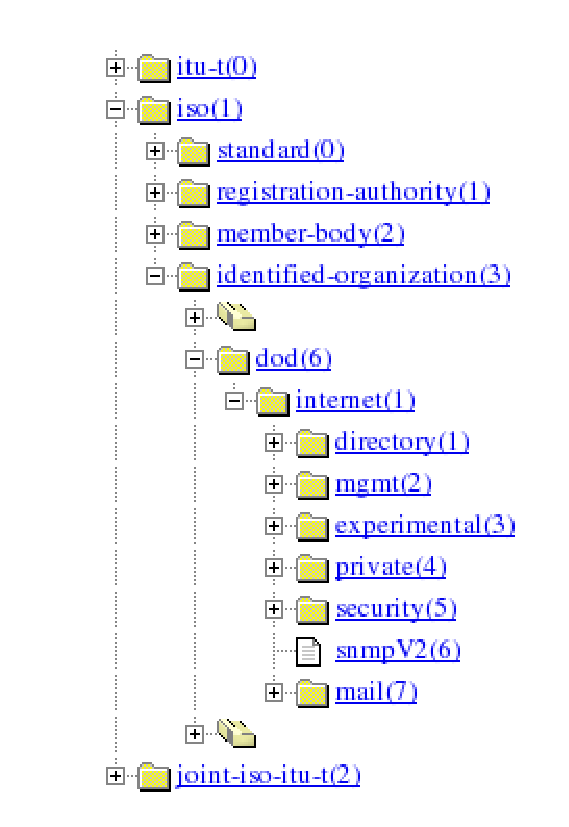
\epsfig{file=figs/mibtree.eps, width=0.35\linewidth}
      % \caption{http://asn1.elibel.tm.fr/cgi-bin/oid/display?tree=1.3.6.1}
    \end{figure}
  \end{floatingfigure}

  \vspace*{.2in}
  \emph{Management Information Base} (MIB) is a 
  formal description of a set of \emph{managed 
  objects} that can be accessed using the Simple  
  Network Management Protocol (SNMP).  The set is 
  arranged in a hierarchical or tree structure. 

  \vspace*{.2in}
  Each managed object is associated with a unique \emph{Object Identifier}, a
  sequence of up to 128 32 bit integers.

  \vspace*{.2in}
  A \emph{MIB module} is a subtree in the MIB, is usually defined by an RFC.
  
\end{slide}



% Structure of MIB tables
\overlays{3}{
\begin{slide}{Structure of MIB tables}
	\vspace*{.2in}

  tcpConnEntry = 1.3.6.1.2.1.6.13.1

  \onlySlide*{1}{
    {\tiny
      \begin{tabular}{|c|c|c|c|c|}
        \multicolumn{5}{c}{tcpConn} \\
        State(\textcolor{OliveGreen}{1}) 
	& LocalAddress(\textcolor{OliveGreen}{2})  
	& LocalPort(\textcolor{OliveGreen}{3})  
	& RemAddress(\textcolor{OliveGreen}{4})
	& RemPort(\textcolor{OliveGreen}{5}) \\
        % Saving space for index	
        &  &  &  & \\
        \hline
        synSent(3)  & 1.2.3.4 & 5  & 6.7.8.9 & 9 \\
	% Saving space for OID 
                    &         &    &         &   \\
        \hline
        closing(10) & 1.2.3.4 & 6 & 7.6.5.4  & 8 \\
	% Saving space for OID
                    &         &   &          &    \\
       \hline
      \end{tabular}
    }
  }

  \onlySlide*{2}{
    {\tiny
      \begin{tabular}{|c|c|c|c|c|}
        \multicolumn{5}{c}{tcpConn} \\
        State(\textcolor{OliveGreen}{1}) 
	& LocalAddress(\textcolor{OliveGreen}{2})  
	& LocalPort(\textcolor{OliveGreen}{3})  
	& RemAddress(\textcolor{OliveGreen}{4})
	& RemPort(\textcolor{OliveGreen}{5}) \\
	% indexes
	& \textcolor{BurntOrange}{index1}
	& \textcolor{BurntOrange}{index2}
	& \textcolor{BurntOrange}{index3}
	& \textcolor{BurntOrange}{index4} \\
        \hline
        synSent(3)  & 1.2.3.4 & 5  & 6.7.8.9 & 9 \\
	% Saving space for OID 
                    &         &    &         &   \\
        \hline
        closing(10) & 1.2.3.4 & 6 & 7.6.5.4  & 8 \\
	% Saving space for OID
                    &         &   &          &    \\
       \hline
      \end{tabular}
    }
  }


  \onlySlide{3}{
    {\tiny
      \begin{tabular}{|c|c|c|c|c|}
        \multicolumn{5}{c}{tcpConn} \\
        State(\textcolor{OliveGreen}{1}) 
	& LocalAddress(\textcolor{OliveGreen}{2})  
	& LocalPort(\textcolor{OliveGreen}{3})  
	& RemAddress(\textcolor{OliveGreen}{4})
	& RemPort(\textcolor{OliveGreen}{5}) \\
	% indexes
	& \textcolor{BurntOrange}{index1}
	& \textcolor{BurntOrange}{index2}
	& \textcolor{BurntOrange}{index3}
	& \textcolor{BurntOrange}{index4} \\
        \hline
        synSent(3)  & 1.2.3.4 & 5  & 6.7.8.9 & 9 \\
        \textcolor{OliveGreen}{.1}\textcolor{BurntOrange}{.1.2.3.4.5.6.7.8.9.9}
        & \textcolor{OliveGreen}{.2}\textcolor{BurntOrange}{.1.2\dots9.9}
        & \textcolor{OliveGreen}{.3}\textcolor{BurntOrange}{.1.2\dots9.9}
        & \textcolor{OliveGreen}{.4}\textcolor{BurntOrange}{.1.2\dots9.9}
        & \textcolor{OliveGreen}{.5}\textcolor{BurntOrange}{.1.2\dots9.9} \\
        \hline
        closing(10) & 1.2.3.4 & 6 & 7.6.5.4  & 8 \\
        \textcolor{OliveGreen}{.1}\textcolor{BurntOrange}{.1.2.3.4.6.7.6.5.4.8}
        & \textcolor{OliveGreen}{.2}\textcolor{BurntOrange}{.1.2\dots4.8}
        & \textcolor{OliveGreen}{.3}\textcolor{BurntOrange}{.1.2\dots4.8}
        & \textcolor{OliveGreen}{.4}\textcolor{BurntOrange}{.1.2\dots4.8}
        & \textcolor{OliveGreen}{.5}\textcolor{BurntOrange}{.1.2\dots4.8} \\
       \hline
      \end{tabular}
    }
  }

  \vspace*{.2in}
  Lexicographical order traversal will be \emph{column centric}.   

\end{slide}
}




% SNMP PDUs
\begin{slide}{SNMPv2 PDUs}

    \textcolor{BurntOrange}{GetRequest, GetNextRequest, SetRequest, Trap,
	Info}
    \begin{tabular}{|c|c|c|c|c|}
    \hline  
    type & id & 0 & 0 & \textcolor{OliveGreen}{variable-bindings} \\
    \hline  
    \end{tabular}

    \vspace*{.2in}
    \textcolor{BurntOrange}{GetBulkRequest}
    \begin{tabular}{|c|c|c|c|c|}
    \hline  
    type & id & non-repeaters & max-repetitions & 
	\textcolor{OliveGreen}{variable-bindings} \\
    \hline  
    \end{tabular}

    \vspace*{.2in}
    \textcolor{BurntOrange}{Response}
    \begin{tabular}{|c|c|c|c|c|}
    \hline  
    type & id & error-status & error-index & 
	\textcolor{OliveGreen}{variable-bindings} \\
    \hline  
    \end{tabular}

    \vspace*{.2in}
    \textcolor{OliveGreen}{variable-bindings}
    \begin{tabular}{|c|c|c|c|c|c|}
    \hline  
    name1 & value1 & name2 & value2 & \dots & size of varbind \\
    \hline  
    \end{tabular}

\end{slide}




% XORP integration with snmpd 
\begin{slide}{XORP integration with snmpd}
    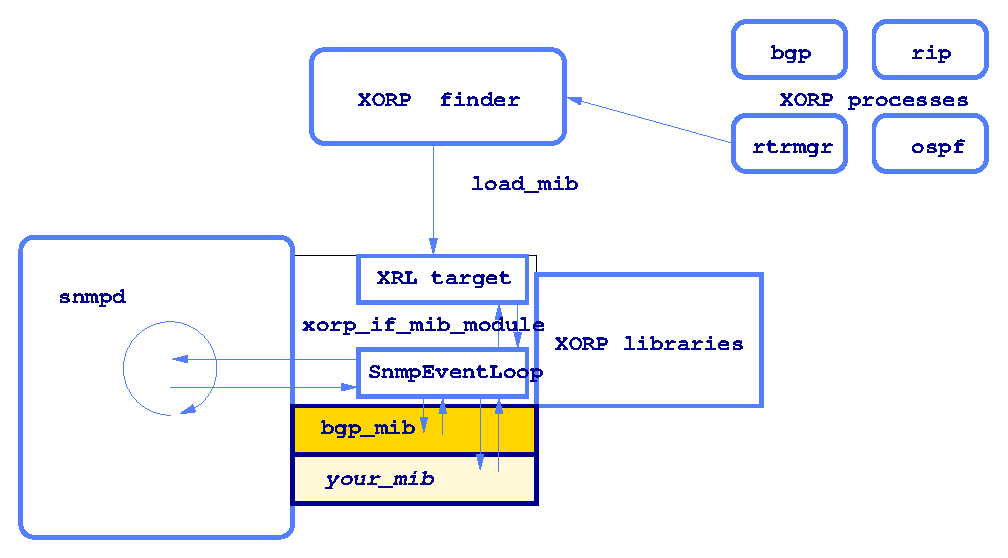
\epsfig{file=figs/snmp_fig2.eps, width=1.05\linewidth}
\end{slide}


% Step by step instructions
\overlays{5}{
\begin{slide}{Step by step instructions}
    \vspace*{.2in}
    \begin{itemstep}
      \item Find (or write) the textual MIB definition file that you want to
            implement. 
      \item Write the derived classes needed to send and process XRLs
      \item Compile your MIB definition file 
      \item Complete the callback functions generated by mib2c
      \item Test your module
    \end{itemstep}
\end{slide}
}



% Finding MIB definition file 
\overlays{2}{
\begin{slide}[Wipe]{Finding the MIB definition file}
	{\large \textcolor{RoyalBlue}{G}\textcolor{RedOrange}{o}\textcolor{Goldenrod}{o}\textcolor{RoyalBlue}{g}\textcolor{OliveGreen}{l}\textcolor{RedOrange}{e}} 
	\fbox{\textbf{<your protocol here>} RFC MIB}
	\vspace{.2in}
\onlySlide{2}{
    {\tiny\texttt{\\
BGP4-MIB DEFINITIONS ::= BEGIN \\
\hspace{.1in}   IMPORTS \\
\hspace{.2in}       MODULE-IDENTITY, OBJECT-TYPE, NOTIFICATION-TYPE, \\
\hspace{.2in}        IpAddress, Integer32, Counter32, Gauge32 \\
\hspace{.2in}           FROM SNMPv2-SMI\\
\hspace{.1in}       mib-2\\
\hspace{.2in}           FROM RFC1213-MIB;\\
\hspace{.1in}   bgp MODULE-IDENTITY\\
\hspace{.2in}       LAST-UPDATED "9405050000Z"\\
\hspace{.2in}       ORGANIZATION "IETF BGP Working Group"\\
\hspace{.2in}       CONTACT-INFO\\
\hspace{.3in}               (...)\\
\hspace{.2in}           DESCRIPTION\\
\hspace{.3in}                   "The MIB module for BGP-4." \\
\hspace{.2in}       ::= \{ mib-2 15 \} \\
    }}
}
\end{slide}
}


% MIB classes
\begin{slide}{Classes needed to process XRLs}
    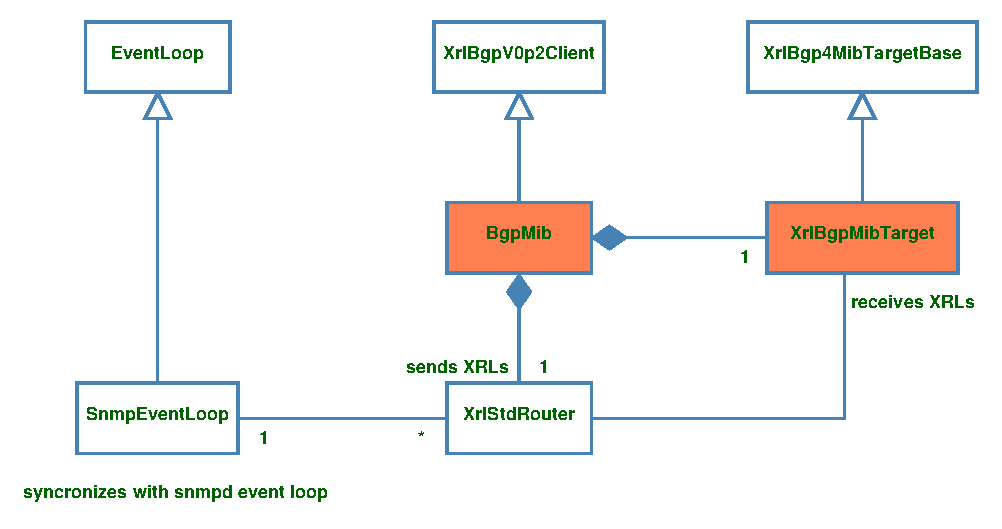
\epsfig{file=figs/bgp_mib.eps, width=\linewidth}
\end{slide}

% Compile your MIB definition file 
\begin{slide}{Compiling your MIB definition file}
  \vspace*{.2in}
  \mbox{\texttt{\$ mib2c -i -c mib2c.iterate.conf -f <fname> <table>}} \\
  \mbox{\texttt{writing to <fname>.c}} \\
  \mbox{\texttt{writing to <fname>.h}} \\
  \vspace*{.2in}
  \mbox{\texttt{\$ mib2c -i -c mib2c.scalar.conf -f <fname> <scalar>}} \\
  \mbox{\texttt{writing to <fname>.c}} \\
  \mbox{\texttt{writing to <fname>.h}} \\
\end{slide}


% Complete the callback functions generated by mib2c
\overlays{3}{
\begin{slide}{Callback functions}
  \begin{itemstep}
  \vspace*{.2in}
    \item \texttt{get\_first\_data\_point} \\
      Create the context required to access your table
      (\emph{loop\_context})
  \vspace*{.2in}
    \item \texttt{get\_next\_data\_point(\emph{loop\_context})} \\
      Despite the misleading name, in this function you should move to the next
      row, and create the context for that row (\emph{data\_context})
  \vspace*{.2in}
    \item \texttt{\emph{table\_name}\_handler(\emph{data\_context,\\
      \hspace{1.7in}column\_number})} \\
      Set the value for the element
  \end{itemstep}
\end{slide}
}

% Test your module
\overlays{4}{
\begin{slide}{Test your module}
  \begin{itemstep}
    \item Start the finder and your protocol process
    \vspace*{.1in}
    \item Configure snmpd so it loads xorp\_if\_mib\_module on startup \\
          by adding the following line to your snmpd.conf\\ 
          \texttt{dlmod xorp\_if\_mib\_module  \\
        \hspace{.2in}/path/to/xorp\_if\_mib\_module.so} 
    \vspace*{.1in}
    \item Start \texttt{snmpd} and send it the XRL to load your MIB\\ 
    \texttt{finder://xorp\_if\_mib/xorp\_if\_mib/0.1/load\_mib\\
      \hspace{.2in}?mod\_name:txt=bgp4\_mib\_1657\\
      \hspace{.2in}\&abs\_path:txt=/path/to/bgp4\_mib\_1657.so
    }
    \vspace*{.1in}
    \item Use one for Net-SNMP client-side commands to read your MIB\\ 
    \texttt{
      snmpwalk localhost bgpPeerTable
    }
  \end{itemstep}
\end{slide}
}

% So how efficient is our MIB access?
\overlays{3}{
\begin{slide}{So how efficient is this approach?}
  \begin{itemstep}
    \vspace*{.2in}
    \item Reading a table with $m$ columns by $n$ rows produces
    \textcolor{Orange} {$O(mn^2)$!!} calls to \texttt{get\_next\_data\_point}.
    \vspace*{.2in}
    \item This is because the algorithm assumes unordered rows.  
    \vspace*{.2in}
    \item Currently working with the Net-SNMP team to improve performance.
  \end{itemstep}
\end{slide}
}

% About atomicity
\begin{slide}{About atomicity}
  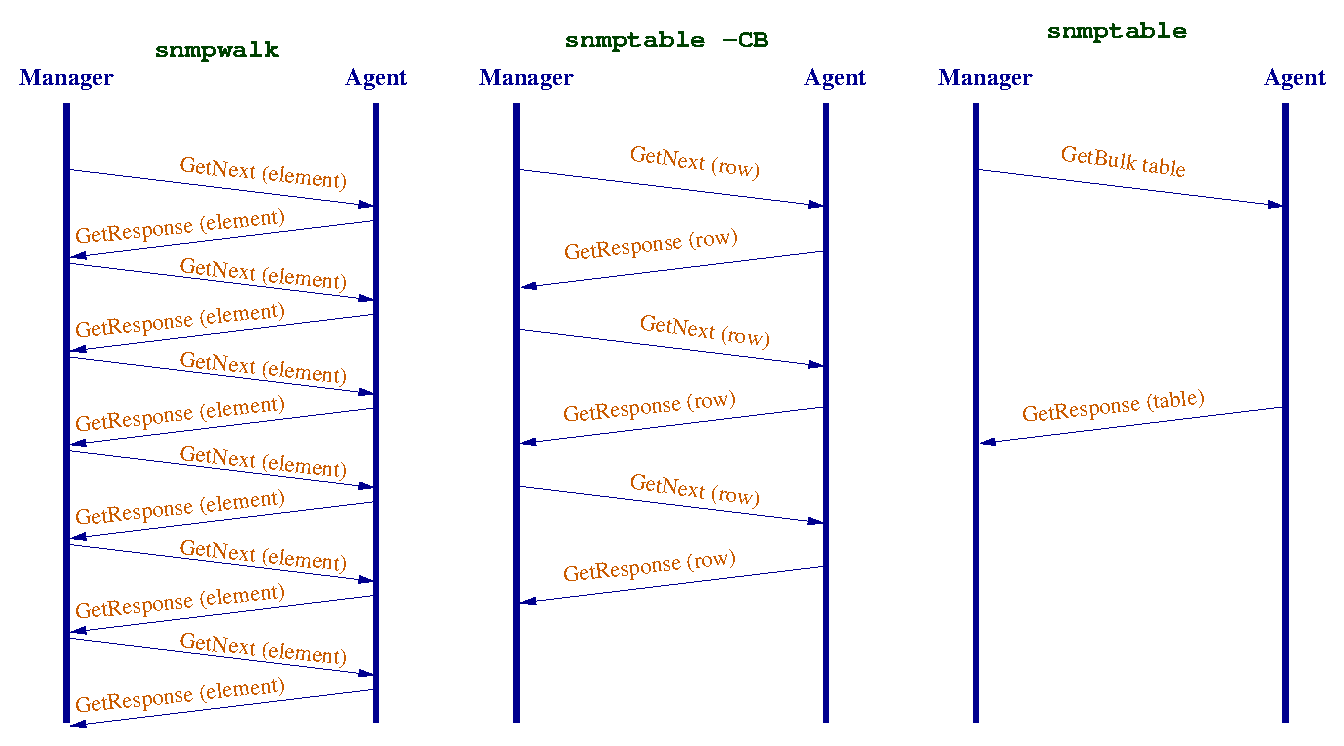
\epsfig{file=figs/pdu_seq.eps, width=\linewidth}
  \begin{tabular}{c @{\hspace{1cm}} c @{\hspace{1cm}} c}
    No way to ensure & Rows should be   & Table should be \\
    consistency      & consistent        & consistent     \\
  \end{tabular}
\end{slide}

% Thank you!!
\overlays{3}{
\begin{slide}{Thank you!}
  \begin{itemstep}
    \vspace{.2in}
    \item for listening
    \vspace{.2in}
    \item for for your intelligent suggestions
    \vspace{.2in}
    \item \ldots and for not falling asleep!
  \end{itemstep}
\end{slide}
}

\end{document}
